% !TeX root = ./jvk-blatt1.tex

\excercise{Programmstart}
\label{ex1}

\begin{Infobox}[How-To: Wie bekomme ich des Projekt]
    \begin{enumerate}[label=\arabic*.]

        \item Nachdem das Zip-File \jvkpackage heruntergeladen wurde, muss man es in einem geeigneten Ordner entpacken.\\
        \textbf{Windows:} Entpacken funktioniert durch einen Rechtsklick auf die Datei und dann durch Klicken auf \fbox{Alle extrahieren...}$\to$\fbox{Extrahieren}.\\
        \textbf{Linux:} Am schnellsten entpackt man ein Zip-File über das Terminal mit dem Befehl:
        \newline\hspace*{\fill}\texttt{\textgreater\ unzip \jvkpackage}\hspace*{\fill}\newline
        \textbf{Apple:} Nachdem man das Zip-File im Finder offen hat, entpackt man es durch einen einfachen Doppelklick.
    \end{enumerate}
\end{Infobox}


\begin{Infobox}[How-To: Projekt Import in Eclipse]
    \begin{enumerate}[label=\arabic*.]
        \item Um ein Projekt zu importieren, klicke zuerst auf \fbox{File} $\to$ \fbox{Import...}.
        \item Wähle in der Auswahl \fbox{Maven} $\to$ \fbox{Existing Maven Projects} oder nutze das Suchfeld oben um \fbox{Existing Maven Projects} zu finden. Klicke dann auf \fbox{Next \textgreater}.
        \item Drücke oben rechts auf \fbox{Browse...} und suche das Verzeichnis, in welchem die Datei \jvkpackage { }entpackt wurde.
        \item Stelle sicher, dass der Projektname im \textit{Projects} Bereich des Fensters auftaucht.
        \item Zu guter Letzt noch auf \fbox{Finish} drücken.
        \item Nachdem sich das Fenster geschlossen hat, siehst du das Projekt im \textit{Package Explorer} links an der Seite.
        \item Damit das Projekt richtig funktioniert, solltet du im \textit{Package Explorer} das Projekt mit einem Rechtsklick auswählen und dann im Kontextmenü \fbox{Maven} $\to$ \fbox{Update Project...} $\to$ \fbox{OK} ausführen.
    \end{enumerate}
\end{Infobox}


\newpage

\begin{enumerate}
    \item
    \begin{itemize}
        \item Öffne die \texttt{Main}-Datei in dem Dateiexplorer auf der linken Seite.
            Navigiere dazu in den \texttt{src/main/java} Ordner und wähle dann das Paket \texttt{de.unistuttgart.informatik.fius.jvk} aus.
        \item Starte als nächstes das Projekt, um zu schauen ob alles klappt.
            Drücke dazu den grünen Play Button $\vartriangleright$ oben.
        \item Wenn du bei der Installation alles richtig gemacht hast, sollten jetzt keine Fehler (roter Text) auftreten.
            Da wir noch nichts programmiert haben, sollte aber auch sonst nichts passieren.
        \begin{center}
            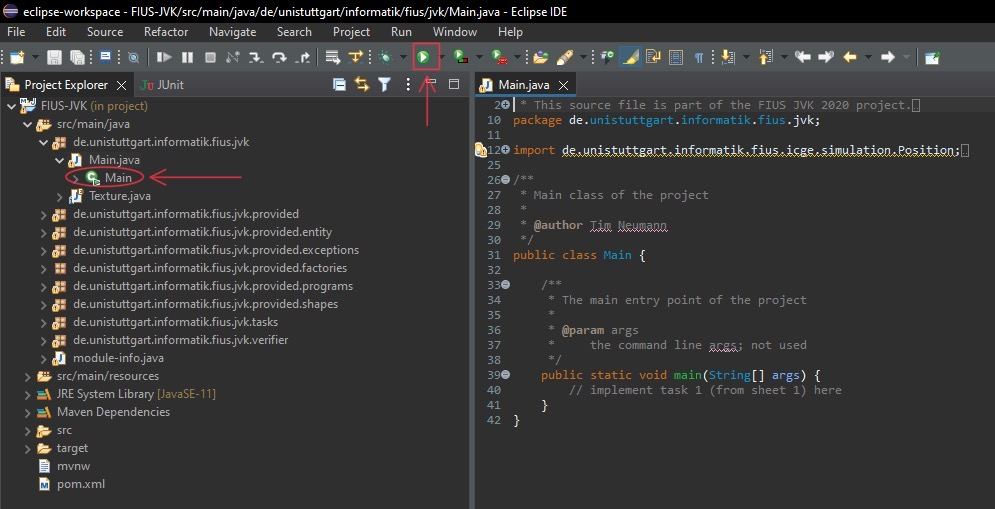
\includegraphics[width=\linewidth]{./figures/ide.jpg}
        \end{center}
    \end{itemize}

    \item Finde in der \lstinline{Main} Klasse die Zeile mit \lstinline{// implement task 1 (from sheet 1) here} und füge an seiner Stelle den fehlenden Code aus dem Bild ein.
    Aktuell musst du den Code noch nicht verstehen, es geht darum den Code Editor in Eclipse kennenzulernen.
    Achte also darauf was passiert während du die fehlenden Zeilen eingibst.

    \begin{lstlisting}
        public class Main {
            /**
            * The main entry point of the project
            *
            * @param args
            *     the command line args; not used
            */
            public static void main(String[] args) {
            // implement task 1 (from sheet 1) here
            Game demoGame = new Game("Hello World", new DemoTask(), new DemoTaskVerifier());
            demoGame.run();
                }
        }   
    \end{lstlisting}

    Wenn das Programm jetzt durch drücken des Play Buttons ausgeführt wird, geht ein Fenster mit der Simulator Ansicht auf.
    Suche als nächstes die (rote) Stop Taste in Eclipse um das Programm abzubrechen.
    Die Taste befindet sich in Eclipse unten in der Titelleiste der Console.
    \item Versuche nun den Code so zu verändern, dass dein Name im Fenstertitel steht.
\end{enumerate}


\begin{Infobox}[Optionale Aufgaben]
    Aufgaben die mit \optional markiert, sind müssen nicht bearbeitet werden.
    Sie setzen schon Vorkenntnisse in Java oder Programmieren voraus und sind deshalb auch oft deutlich schwerer als die normalen Aufgaben.
    Wenn du also an einer optionalen Aufgabe festhängst, dann solltest du mit der nächsten normalen Aufgabe weitermachen.
    Später, wenn du genug Zeit oder Wissen hast um die optionale Aufgabe zu lösen, kannst du nochmal zu ihr zurückkehren.
\end{Infobox}


\begin{enumerate} \setcounter{enumi}{3}
\item \optional Finde eine Möglichkeit, den Fenstertitel nach der \lstinline{demoGame.run();} Zeile zu ändern.
Dafür benötigst du den folgenden Code, den du aber noch auf deinen Namen anpassen musst: \lstinline{demoGame.getGameWindow().setWindowTitle("");}
\item \optional Versuche, drei Fenster gleichzeitig zu starten.
\end{enumerate}
